\section{Anwendungsgebiete von AR}

\subsection{Archäologie}

Die Technologie der Augmented Reality (“Erweiterte Realität”, AR) findet in der Archäologie Anwendung, insbesondere im Bereich des erweiterten Tourismus. Sie zielt darauf ab, die Erfahrung des Besuchs historischer Stätten zu verbessern, indem virtuelle Rekonstruktionen über die reale Umgebung gelegt werden. Dies wird durch den Einsatz von Geräten wie Head Mounted Displays (HMDs) oder mobilen Geräten erreicht, die virtuelle Objekte über Live-Videoübertragungen legen. Bemerkenswerte Beispiele für diese Technologie sind “ARCHEOGUIDE” und das Projekt “Cultural Heritage Experiences through Socio personal Interactions and Storytelling”.

Über den virtuellen Tourismus hinaus kann AR auch helfen, archäologische Stätten aus einer phänomenologischen Perspektive zu erkunden. Durch die Überlagerung von geografischen Daten aus einem Geografischen Informationssystem (GIS) mit der realen Welt wird eine verkörperte Erfahrung der Landschaft ermöglicht. Dieses Konzept wird anhand eines Projekts in einer bronzezeitlichen Siedlung in Cornwall, Grossbritannien, demonstriert, bei dem eine massstabsgetreue Rekonstruktion der Rundhäuser der Siedlung mit Hilfe einer Spiele-Engine, GIS-Software, einem AR-Plugin und benutzerdefinierten Skripten über die reale Landschaft gelegt wurde. 
\cite{Archaeology}

\subsection{Übersetzung}

Die Technologie der Augmented Reality (“Erweiterte Realität”, AR) wird in vielen Anwendungen eingesetzt, wobei die Übersetzung eine ihrer Anwendungen ist. Ein Beispiel, mit dem viele Menschen vielleicht vertraut sind, aber nicht wissen, dass dort eine AR-Technologie verwendet wird, ist die Word Lens Mobile App, die von Google übernommen und in Google Translate integriert wurde. Mit dieser App können die Nutzer einfach ihre Smartphone-Kamera auf Texte wie Schilder oder Speisekarten richten und bekommen sofort eine Übersetzung neben dem Originaltext auf dem Bildschirm angezeigt. Damit entfällt die Notwendigkeit, ein Foto zu machen oder den Text manuell in die App einzugeben, was für Reisende und Sprachschüler auf der ganzen Welt, die Sprachen verstehen und mit ihnen interagieren wollen, äusserst praktisch ist. \cite{QuestVisual_2010}

\vspace{1cm}

\begin{figure}[ht!]
    \centering
    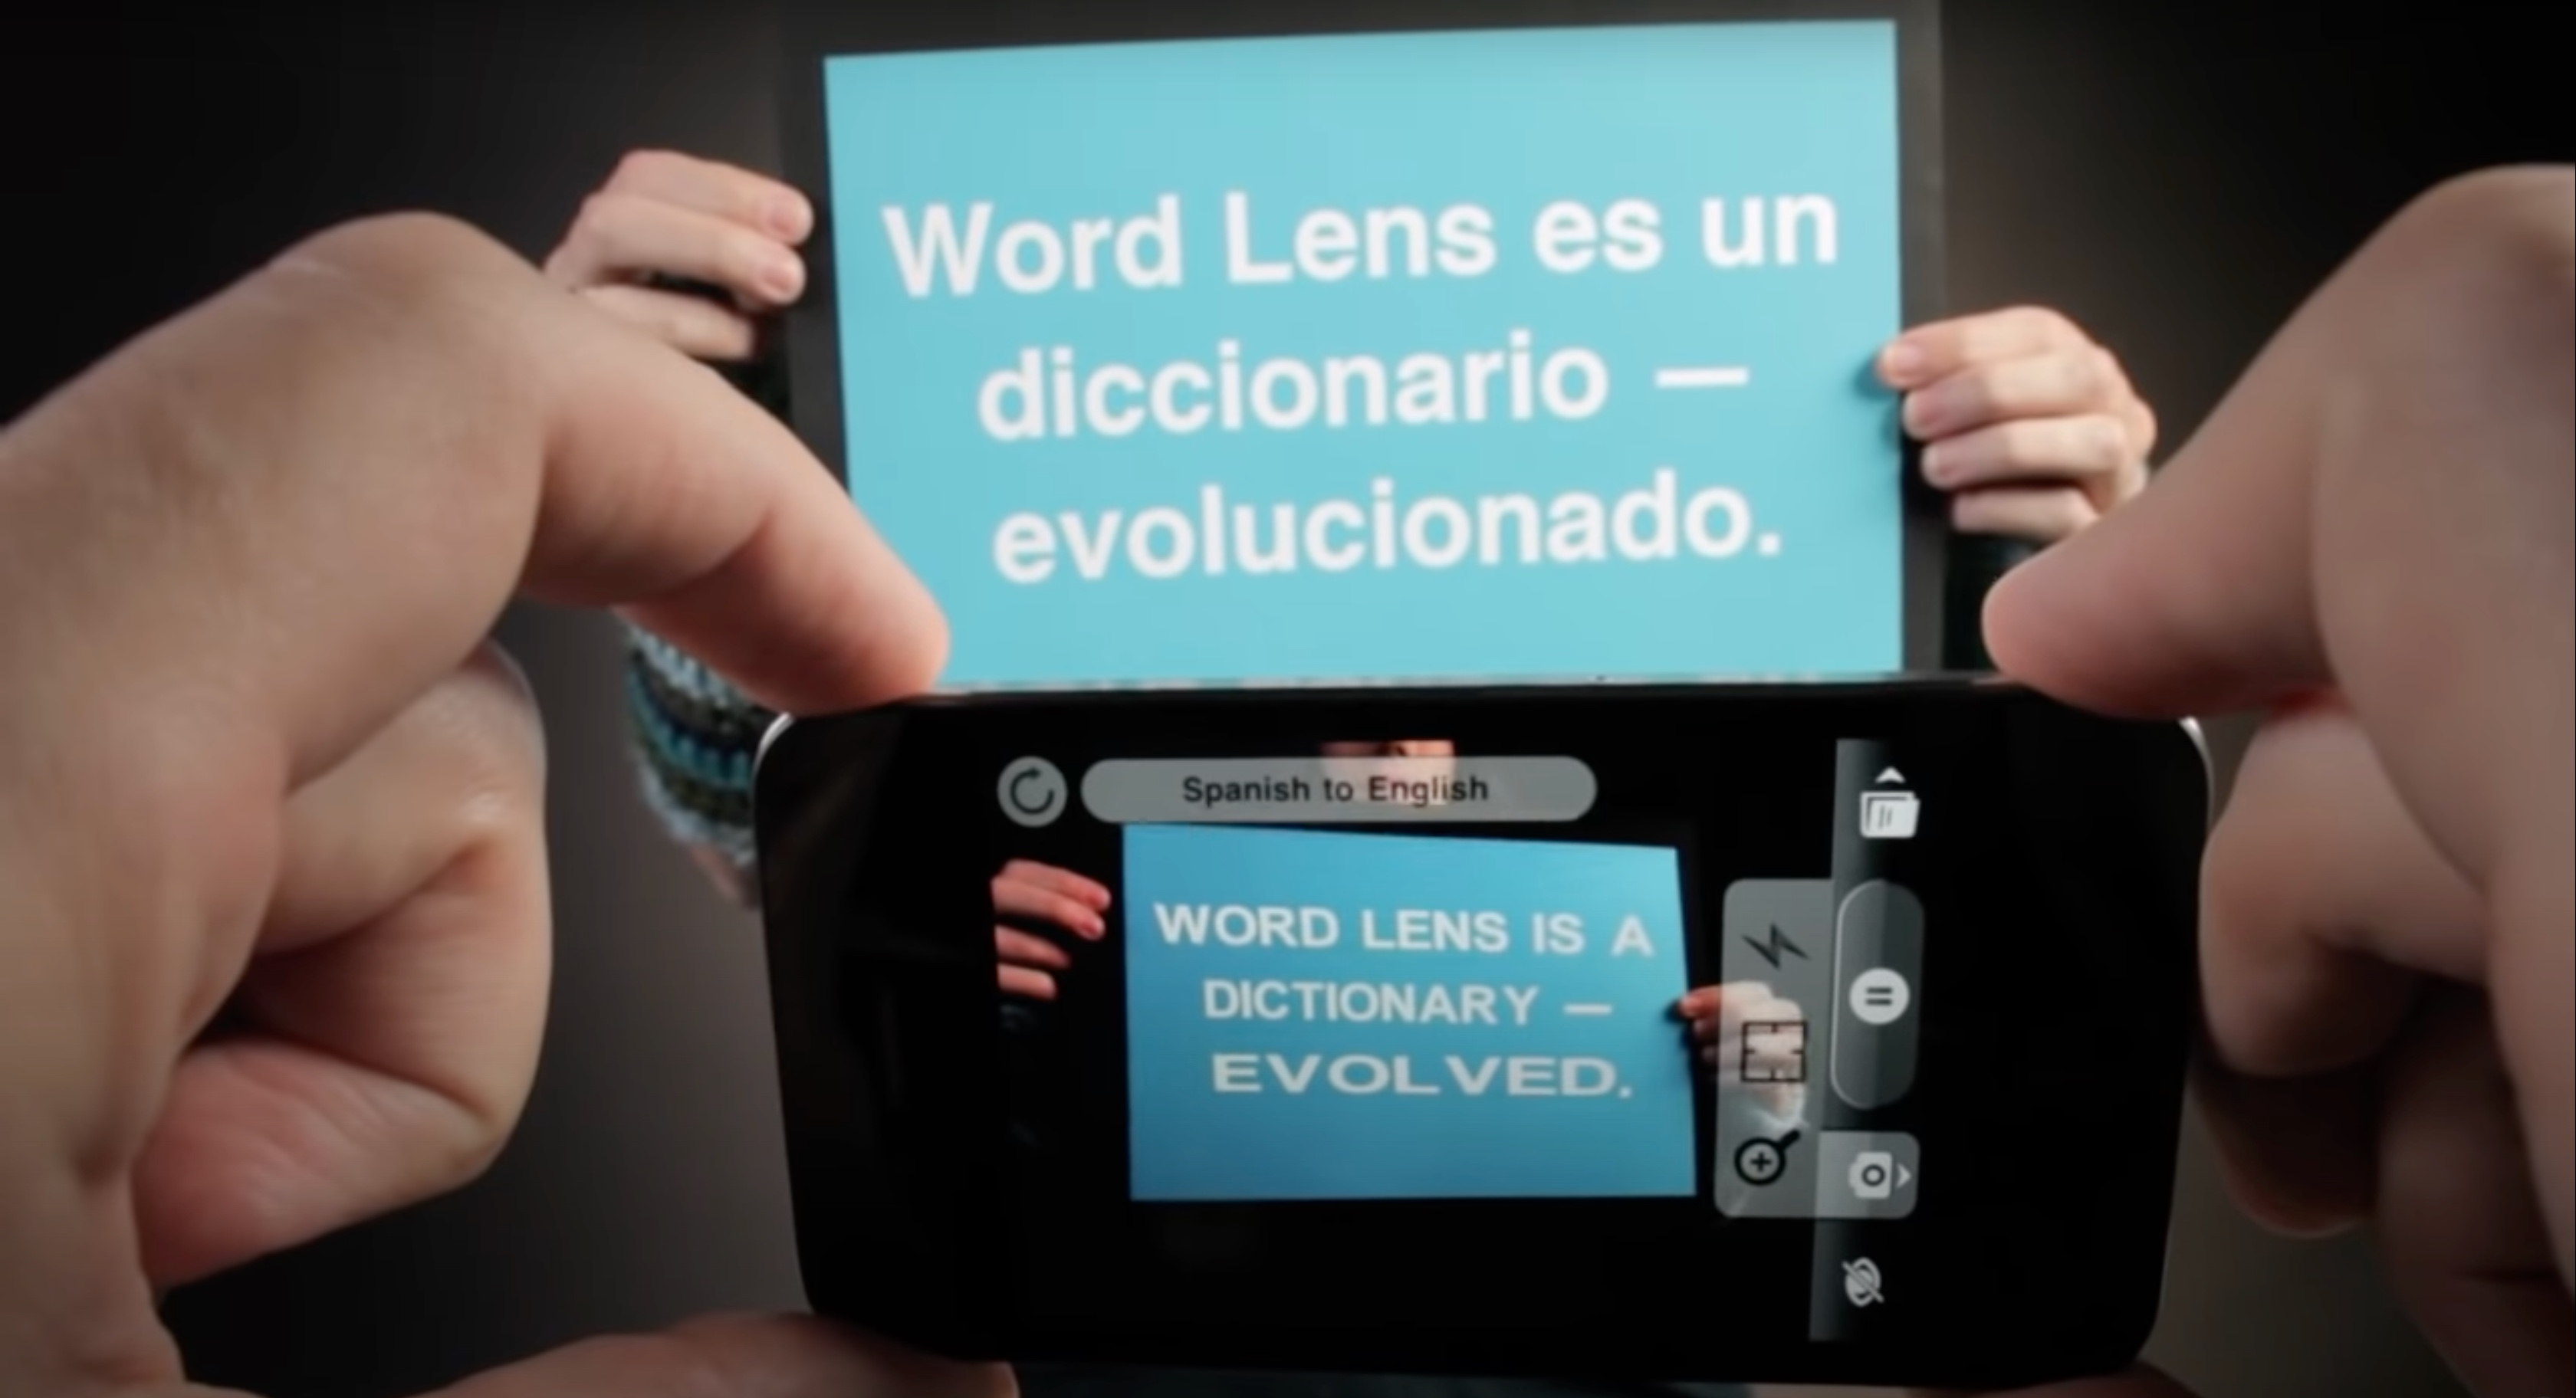
\includegraphics[width=0.7\textwidth]{attachments/Lens.jpeg}
    \caption{Demonstration der Funktionsweise der World Lens} \cite{QuestVisual_2010}
\end{figure}


\subsection{Bildungsbereich}

Augmented Reality (AR) hat das Potenzial, die Bildung durch die Schaffung immersiver Lernumgebungen erheblich zu verändern. Diese Umgebungen ermöglichen es den Lernenden, mit Objekten und Informationen in der realen Welt zu interagieren, was eine praktische und fesselnde Lernerfahrung ermöglicht. AR kann nahtlos in Aktivitäten wie Simulationen, Spiele und Prüfungen integriert werden, um die Entwicklung von kognitiven, emotionalen und physischen Fähigkeiten zu unterstützen. Darüber hinaus bietet AR personalisierte und adaptive Lernerfahrungen, die auf die spezifischen Bedürfnisse der Lernenden zugeschnitten sind und das Interesse, die Motivation und die Zusammenarbeit unter den Schülern fördern. Die pädagogischen Vorteile von AR sind zahlreich, da sie das Behalten von Wissen, die Problemlösungsfähigkeit und die Entscheidungsfindung verbessern und gleichzeitig Kreativität und Innovation fördern. \cite{Wu2013CurrentSO}

Allerdings muss man sich darüber im Klaren sein, dass die Integration von AR in den Unterricht auch mit Herausforderungen verbunden ist. Zu diesen Herausforderungen gehören die Notwendigkeit einer geeigneten Hardware- und Software-Infrastruktur sowie die fehlende Standardisierung verschiedener Plattformen oder Kompatibilitätsprobleme zwischen Systemen oder Geräten. Darüber hinaus besteht die Gefahr, dass die Lernergebnisse beeinträchtigt werden, wenn die Implementierung von AR nicht durchdacht konzipiert oder effektiv durchgeführt wird. Daher müssen Pädagogen und Designer verschiedene Ansätze sorgfältig abwägen und dabei die ethischen Bedenken im Zusammenhang mit dem Einsatz von AR im Bildungsbereich im Auge behalten. Auf diese Weise können sie Strategien und Leitlinien entwickeln, die den Nutzen der erweiterten Realität im Bildungsbereich maximieren.\cite{Wu2013CurrentSO}

\vspace{1cm}

\begin{figure}[h!]
    \centering
    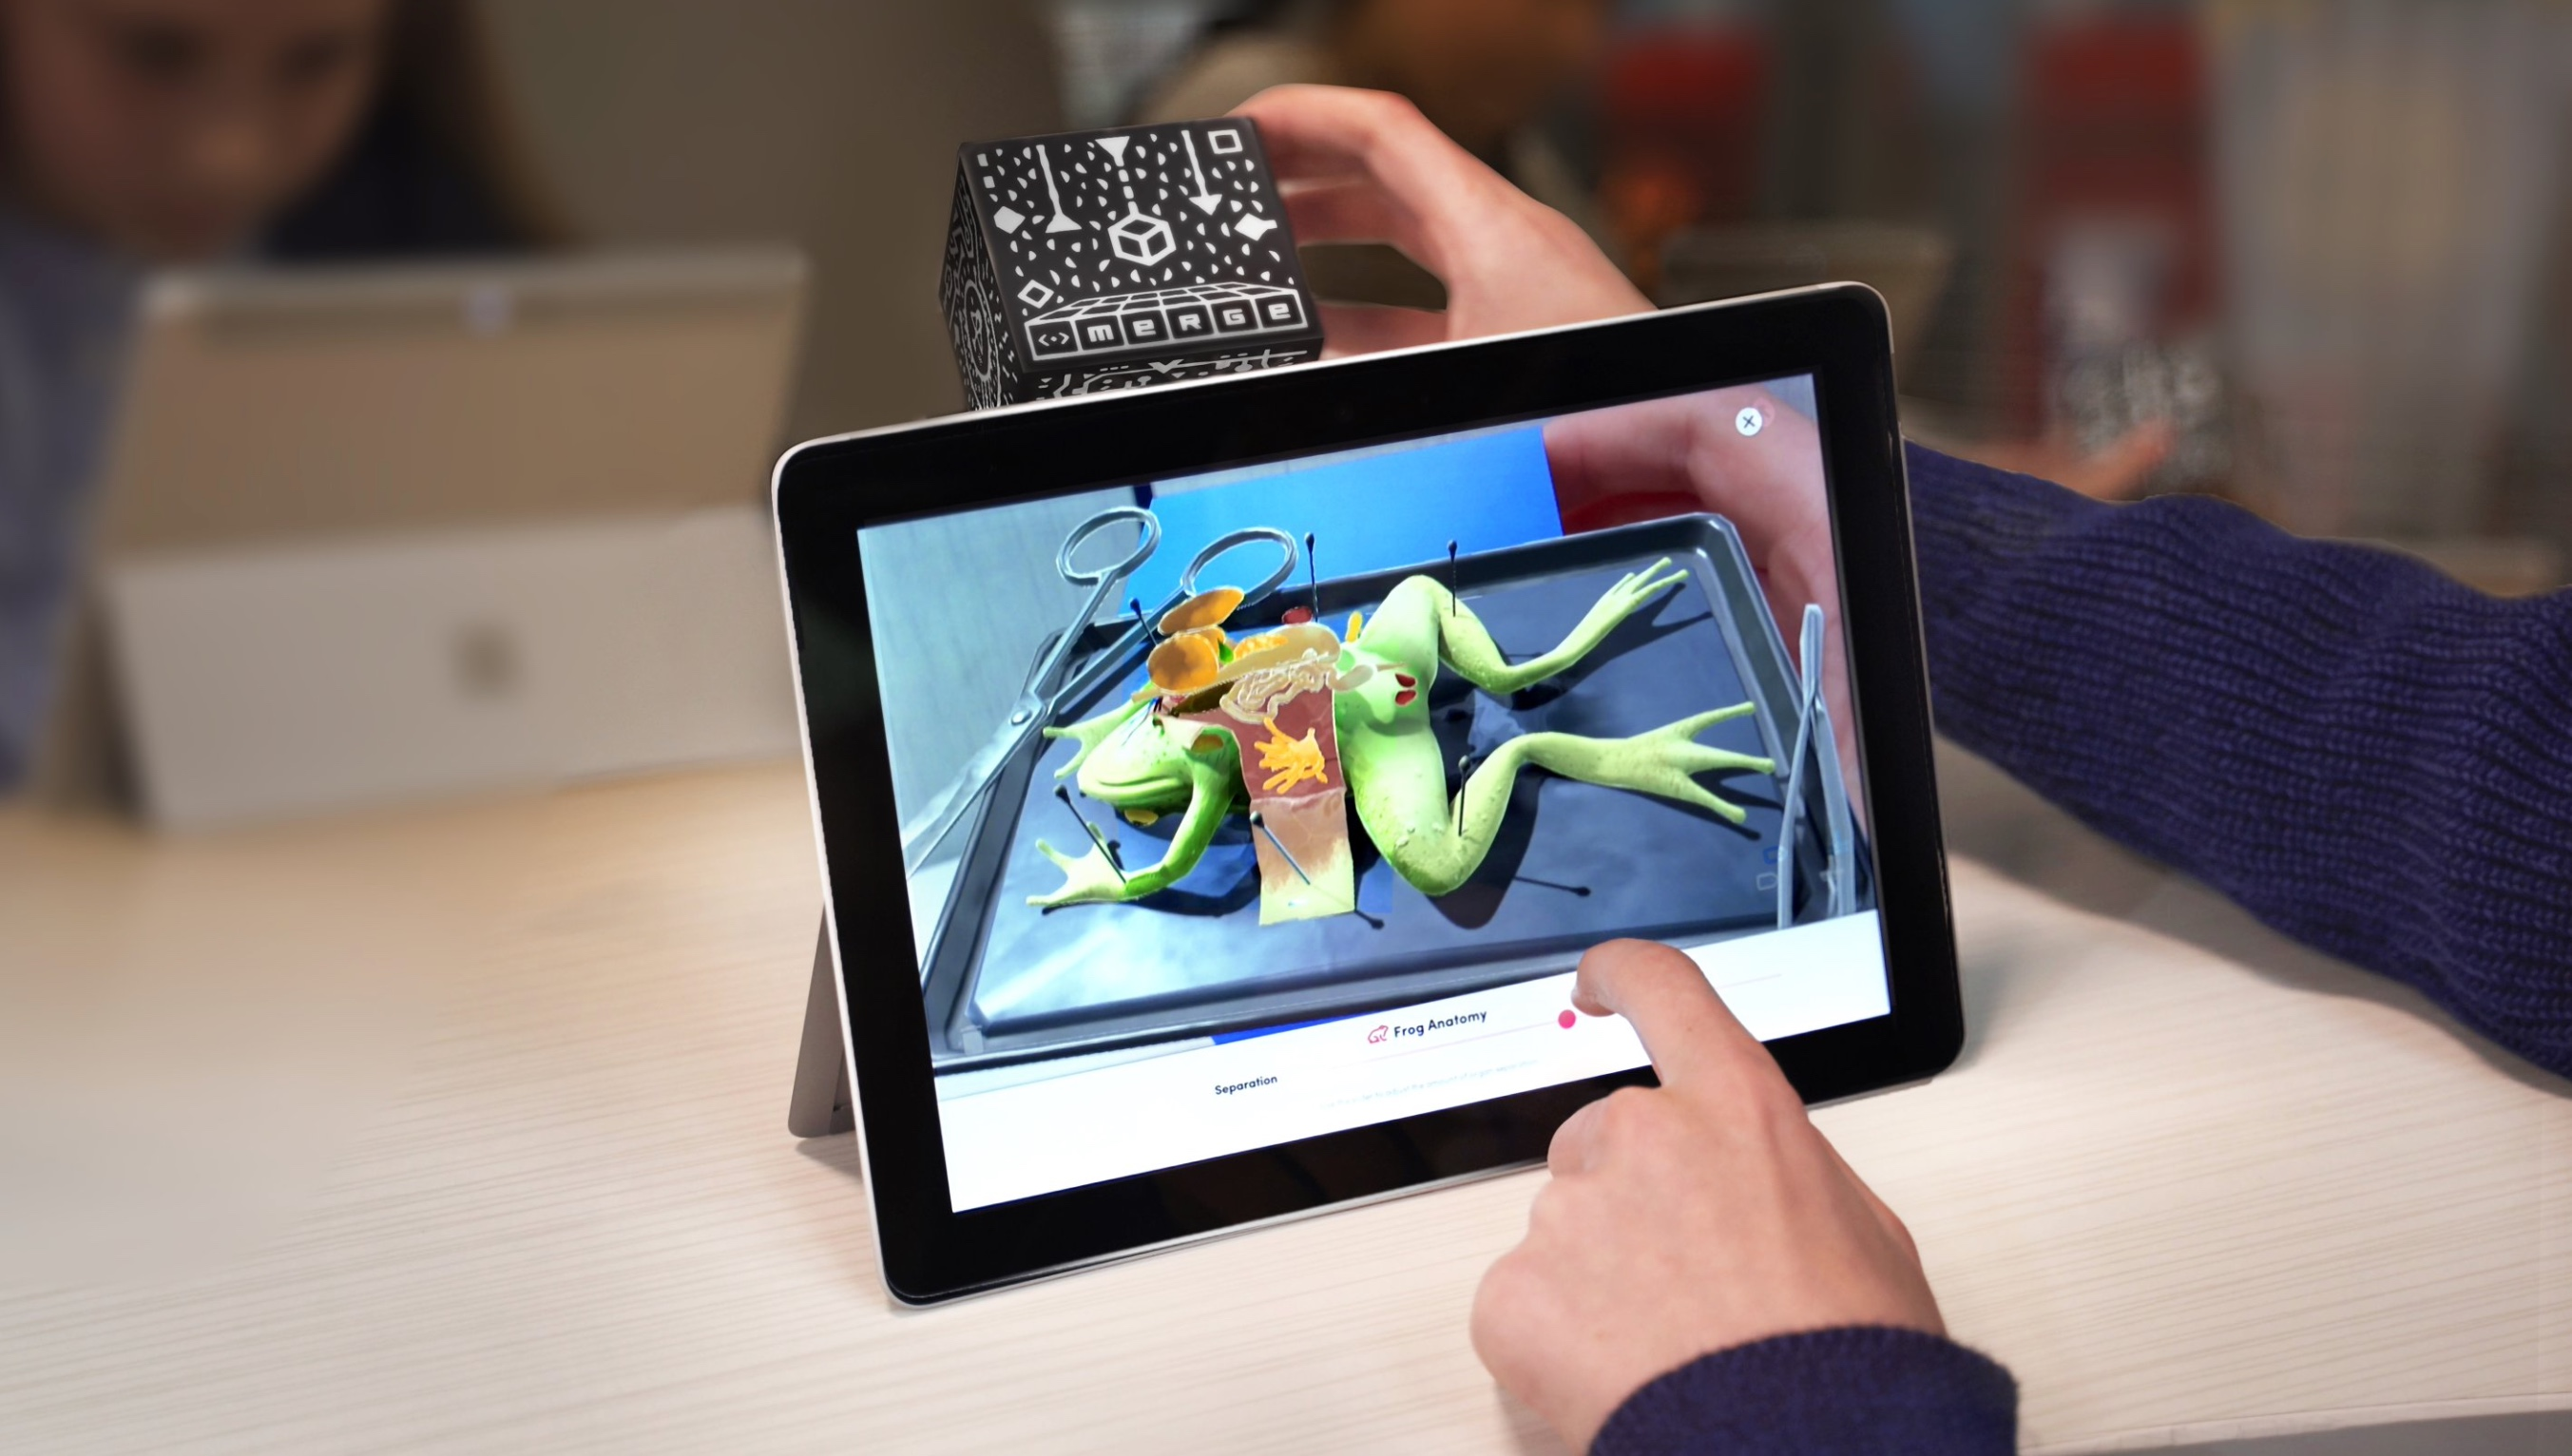
\includegraphics[width=0.7\textwidth]{attachments/cube.jpeg}
    \caption{Schulorientiertes AR-Gerät von Merge EDU} \cite{Merge_EDU}
\end{figure}

\subsection{Videospiele}

Einer der Hauptvorteile der Augmented-Reality-Technologie (AR) in der Videospielindustrie besteht darin, dass sie es den Nutzern ermöglicht, mit synthetischen Objekten, Personen und Umgebungen zu interagieren, die über reale Umgebungen gelegt werden, und ihre Erfahrungen in diesen Umgebungen mit computergenerierten Bildern und Tönen zu erweitern. Dies verbessert das Spielerlebnis und schafft neue Möglichkeiten der sozialen Interaktion. AR-Spiele wie Pokémon GO, Ingress und Zombies, Run! sind bekannte Beispiele für diese Technologie in Aktion. Die körperliche Bewegung, die diese Spiele erfordern, kann jedoch ein Risiko für die Nutzer darstellen, insbesondere wenn sie nicht sicher und verantwortungsvoll genutzt werden. Insgesamt hat AR das Potenzial, die Spieleindustrie zu verbessern und neue und aufregende Erlebnisse für die Spieler zu schaffen. \cite{Das2017AugmentedRV}

\vspace{1cm}

\begin{figure}[ht!]
    \centering
    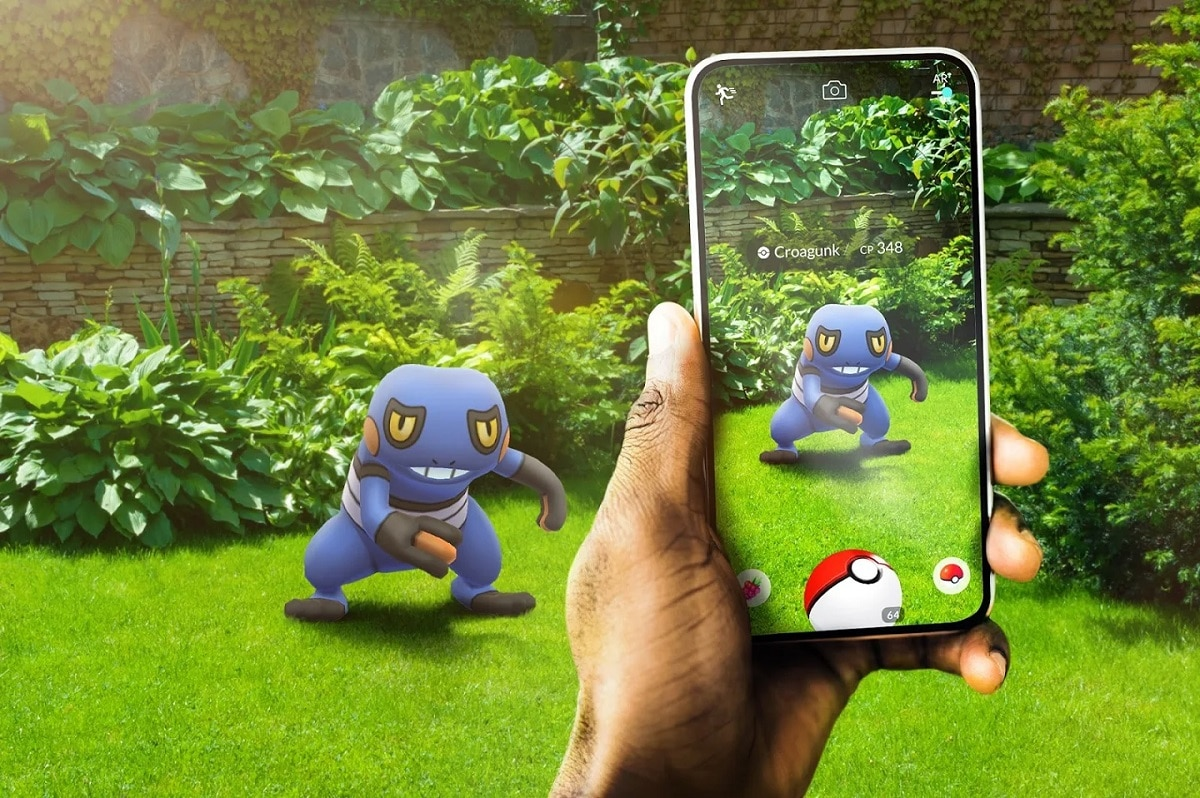
\includegraphics[width=0.7\textwidth]{attachments/pokemon.jpg}
    \caption{AR-Technologie in Pokemon Go verwendet} \cite{Pokemon_GO}
\end{figure}


\subsection{Medizin}
Die Technologie der Augmented Reality (“Erweiterte Realität”, AR) findet in der Praxis Anwendung. Sie ermöglicht die Schaffung von immersiven Lernerfahrungen für Studenten, die komplexe medizinische Konzepte und Verfahren besser verstehen können. \cite{Parsons2021CurrentPO}

Darüber hinaus kann AR Operationen und andere medizinische Verfahren simulieren und so eine kontrollierte Umgebung schaffen, in der die Studenten üben und ihre Fähigkeiten verbessern können. \cite{Parsons2021CurrentPO}

Ausserdem kann Augmented Reality während eines chirurgischen Eingriffs Bilder über den Körper des Patienten legen und dem Chirurgen Anweisungen und Informationen in Echtzeit liefern. Dies trägt dazu bei, die Genauigkeit zu verbessern und Komplikationen bei Operationen zu verringern. \cite{Parsons2021CurrentPO}

AR kann auch eingesetzt werden, um Rehabilitationsprogramme für Patienten zu entwickeln, die sich von Verletzungen oder Operationen erholen. Durch die Bereitstellung von Feedback und Anleitungen werden die Patienten bei der Durchführung von Übungen unterstützt und ihre Fortschritte werden im Laufe der Zeit verfolgt. \cite{cavalcanti2018usability}

Schliesslich spielt Augmented Reality auch eine Rolle bei der Beratung und Unterstützung. Sie ermöglicht es Ärzten, mit Patienten zu interagieren, auch wenn sie räumlich weit voneinander entfernt sind. \cite{Hsieh2018PreliminarySO}

\vspace{1cm}

\begin{figure}[h!]
    \centering
    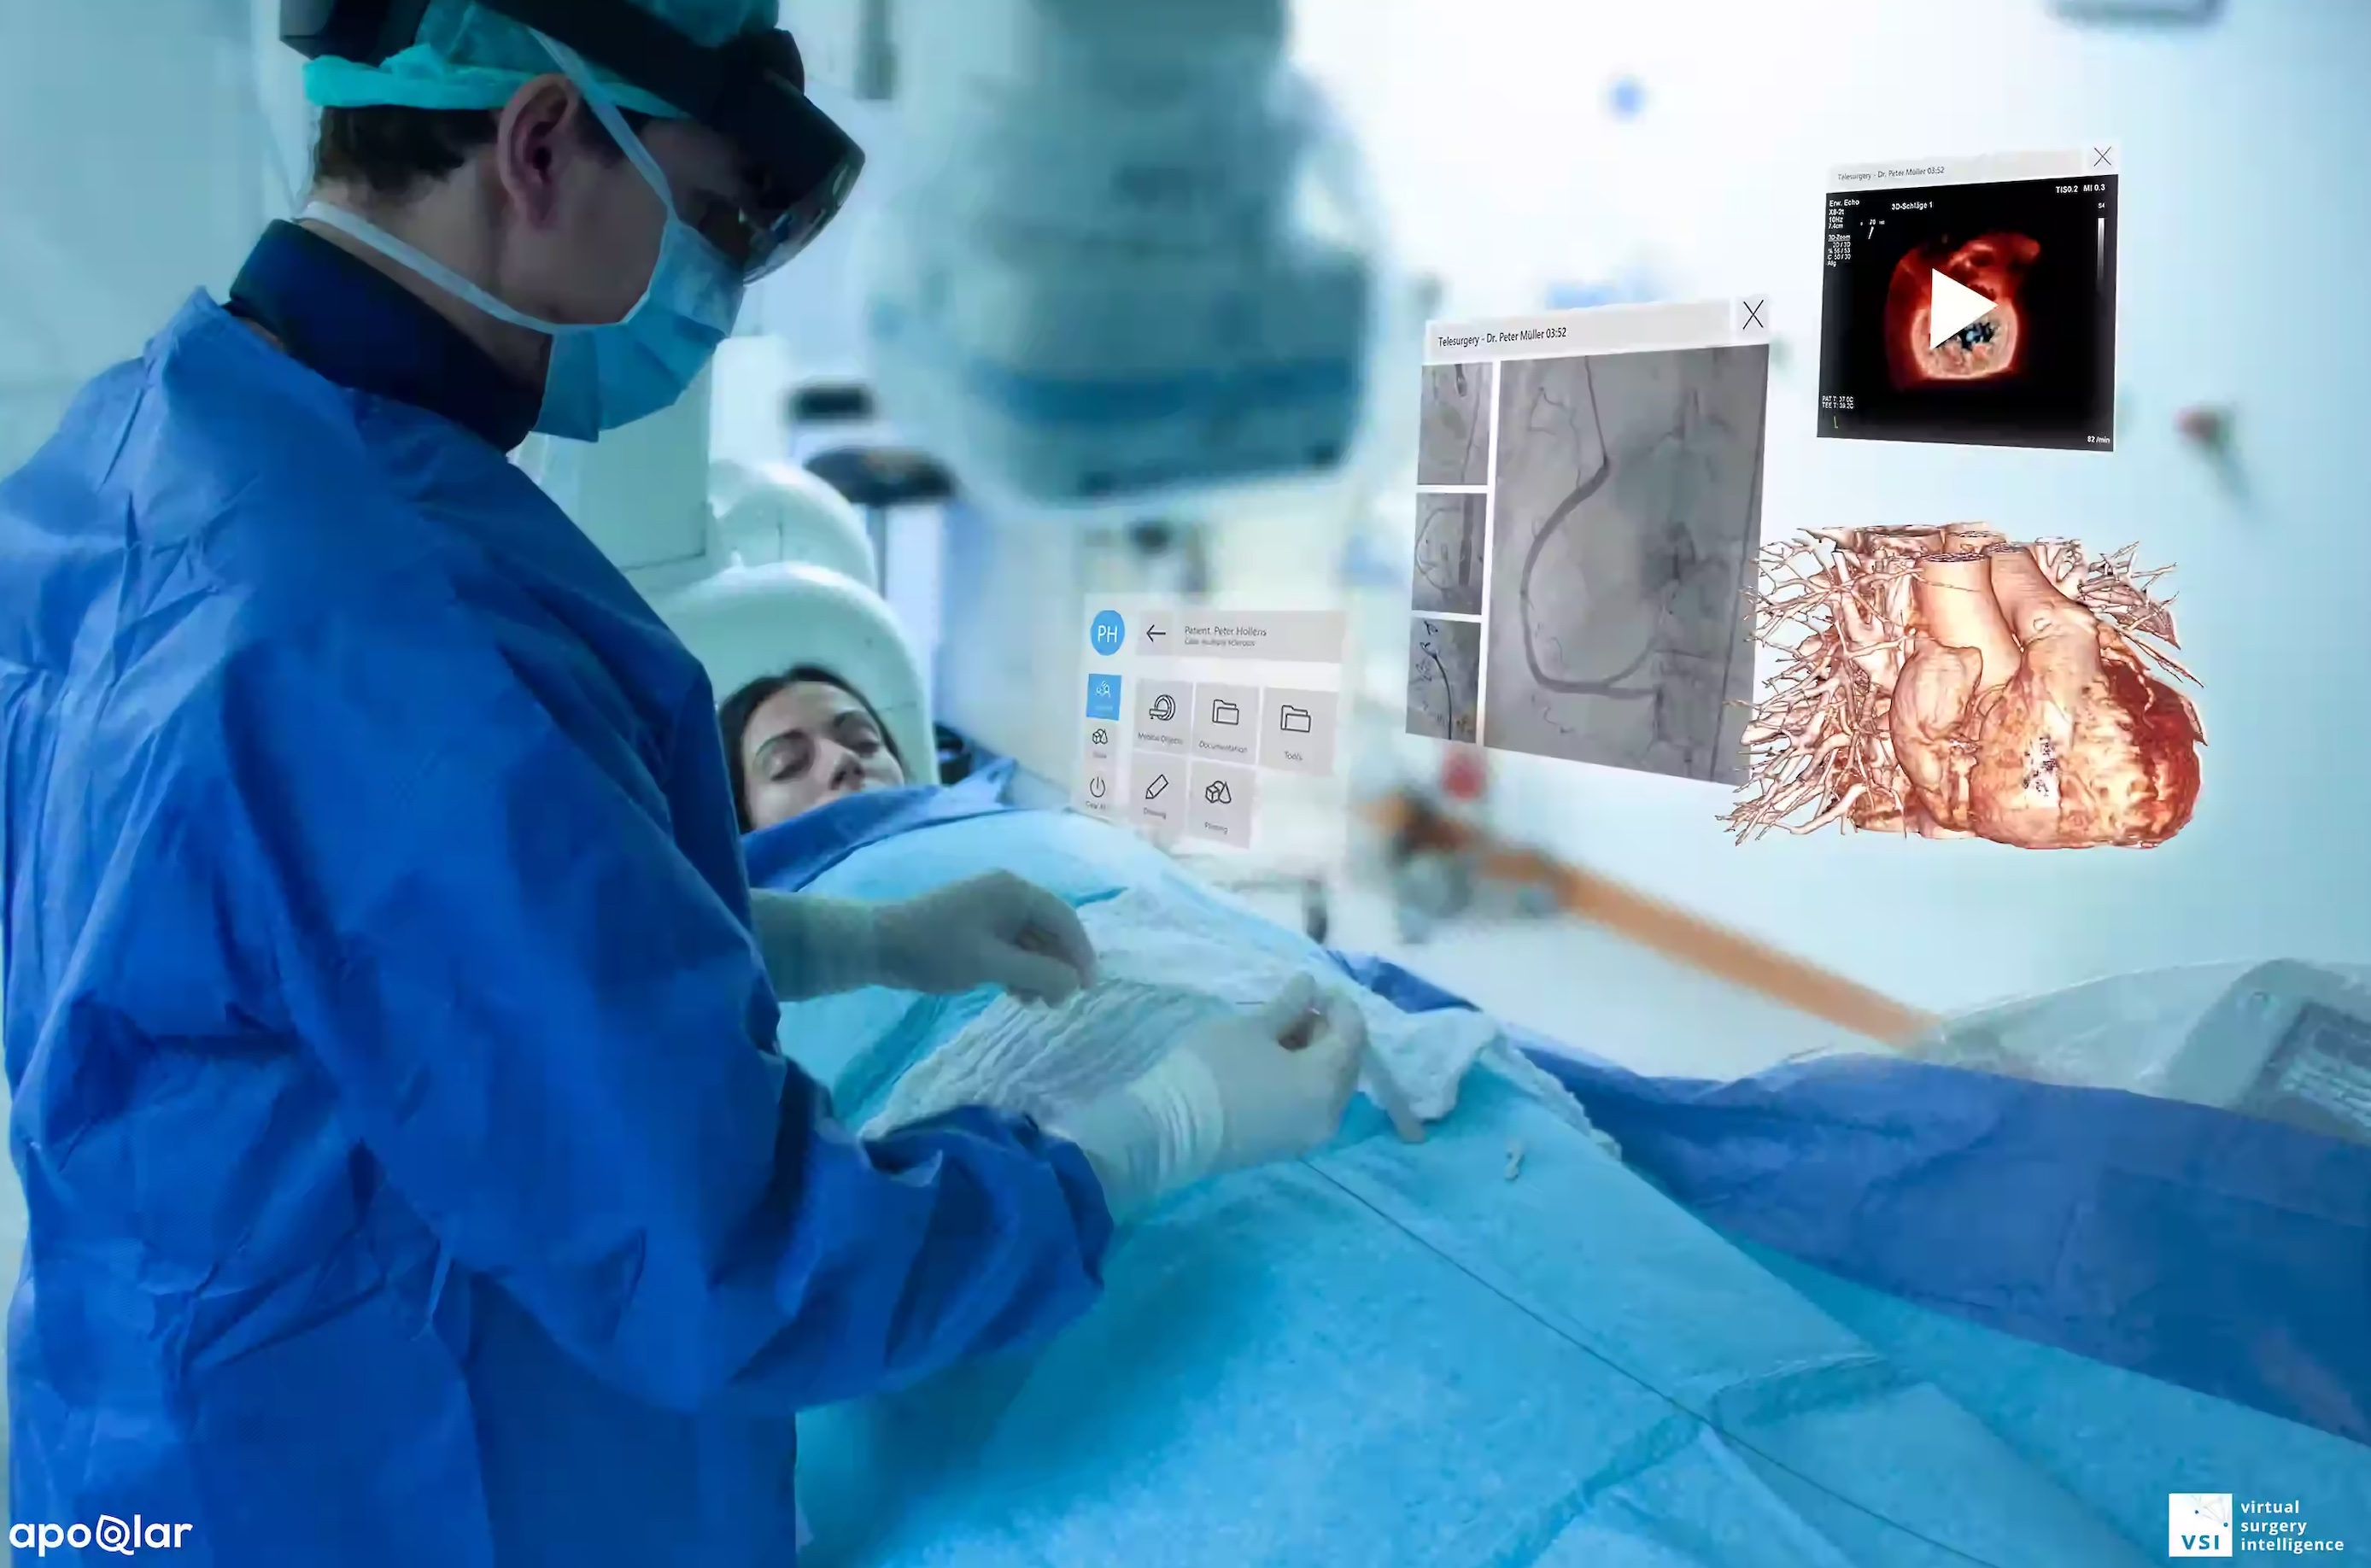
\includegraphics[width=0.7\textwidth]{attachments/surgery.jpeg}
    \caption{Microsoft HoloLens während des Betriebs verwendet} \cite{Microsoft_Healthcare}
\end{figure}

\newpage

\subsection{Militär}
Die AR-Technologie wird auch im Militär eingesetzt, wobei Beispiele aus der realen Welt ihre Wirksamkeit zeigen. Ein Beispiel ist die Nutzung in der Ausbildung, wo sie an der Armeeakademie eingesetzt wurde, um Szenarien zu erstellen, die es Studenten ermöglichen, Trainingssituationen für Bediener zu simulieren und zu modellieren. \cite{Virca2021ApplicationsOA}

Ein weiterer Anwendungsfall ist die Verbesserung des Bewusstseins, wobei Augmented Reality dem Personal Informationen in Echtzeit liefern kann. Diese Echtzeitdaten haben das Potenzial, den gesamten Lebenszyklus militärischer Operationen und die Handlungen des Personals zu begleiten. Darüber hinaus wurden AR-Technologien als kostengünstige Lösung zur Verbesserung der Ausbildung von Soldaten identifiziert. Durch den Einsatz von AR-Technologien können Trainingsprogramme auf die individuellen Bedürfnisse der Soldaten zugeschnitten werden. Darüber hinaus können AR-Technologien computergenerierte Bilder über die Umgebung legen, was die Planung von Operationen erleichtert. \cite{Virca2021ApplicationsOA}

Zusammenfassend lässt sich sagen, dass AR-Technologien die Effizienz von Aktivitäten und Operationen verbessern können, indem sie das Bewusstsein schärfen und dem Personal Informationen in Echtzeit liefern. \cite{Virca2021ApplicationsOA}


\begin{figure}[h!]
    \centering
    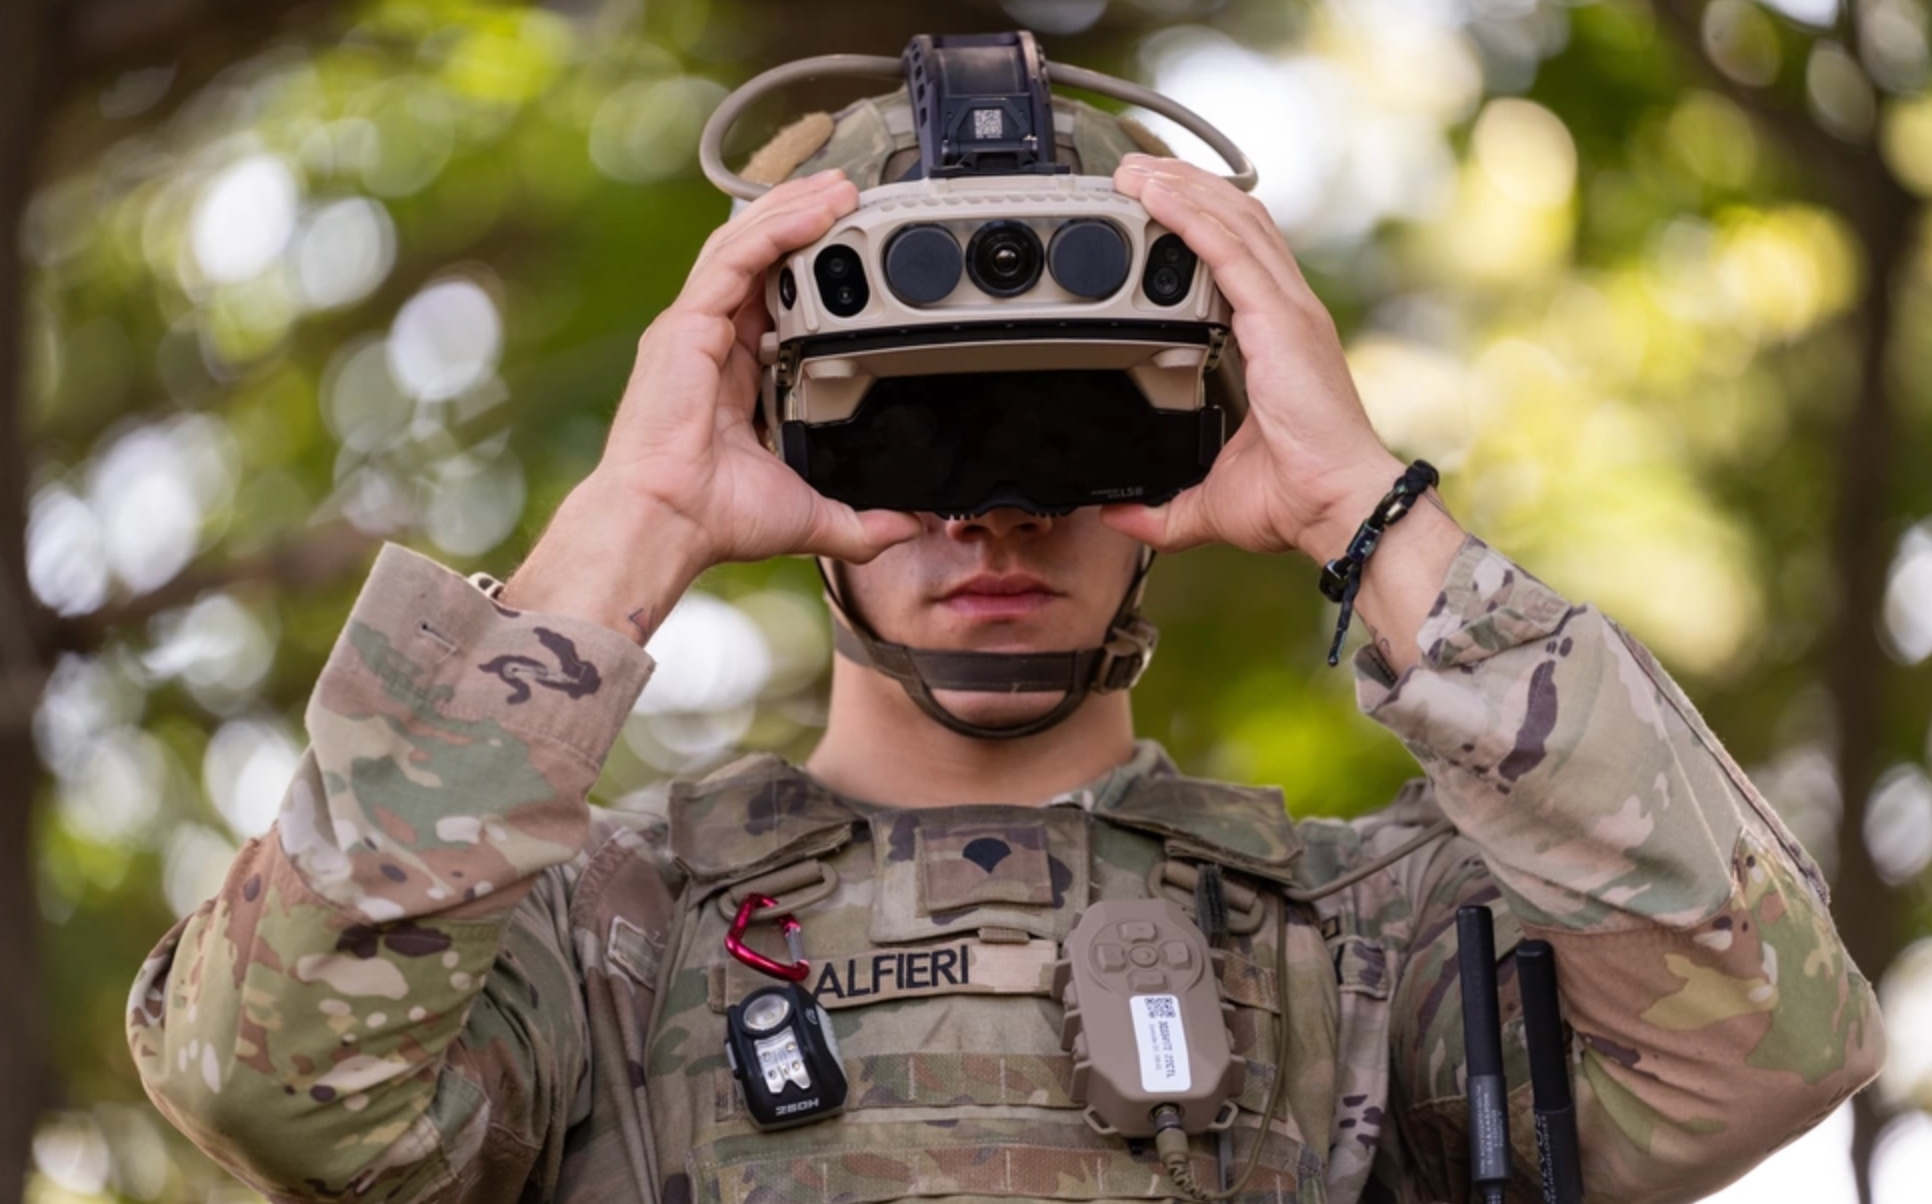
\includegraphics[width=0.5\textwidth]{attachments/army.jpeg}
    \caption{Das Integrated Visual Augmentation (IVAS) System der US-Armee} \cite{Soldier_IVAS}
\end{figure}

\subsection{Navigation}
Wie bereits im geschichtlichen Teil dieses Artikels erwähnt, verwendete das NASA-Raumschiff X-38 ein hybrides System für künstliches Sehen. Dieses System überlagerte Videobilder mit Kartendaten, um die Navigationsfähigkeiten des Raumfahrzeugs zu verbessern. Es basierte auf der Software LandForm, die sich besonders bei schlechten Sichtverhältnissen bewährte. \cite{Delgado2001HybridSS}

Darüber hinaus kann Augmented Reality (AR) zur Verbesserung von Navigationssystemen eingesetzt werden, indem virtuelle Objekte in die reale Welt eingeblendet werden, was zu einer realistischeren und benutzerfreundlicheren Erfahrung führt. AR kann den Nutzern intuitivere und realistischere Navigationsanweisungen geben, z. B. durch Hervorheben von Orientierungspunkten oder Einblenden von Pfeilen in das Sichtfeld des Nutzers. AR kann auch die Sicherheit erhöhen, da der Nutzer seine Aufmerksamkeit nicht mehr von der Strasse ablenken muss. Das Schweizer Unternehmen Way Ray hat beispielsweise holografische AR-Navigationssysteme entwickelt, bei denen holografische optische Elemente verwendet werden, um alle streckenbezogenen Informationen, einschliesslich Wegbeschreibungen, wichtige Mitteilungen und interessante Punkte, direkt in das Sichtfeld des Fahrers und weit vor das Fahrzeug zu projizieren. \cite{WayRay}


\begin{figure}[ht!]
    \centering
    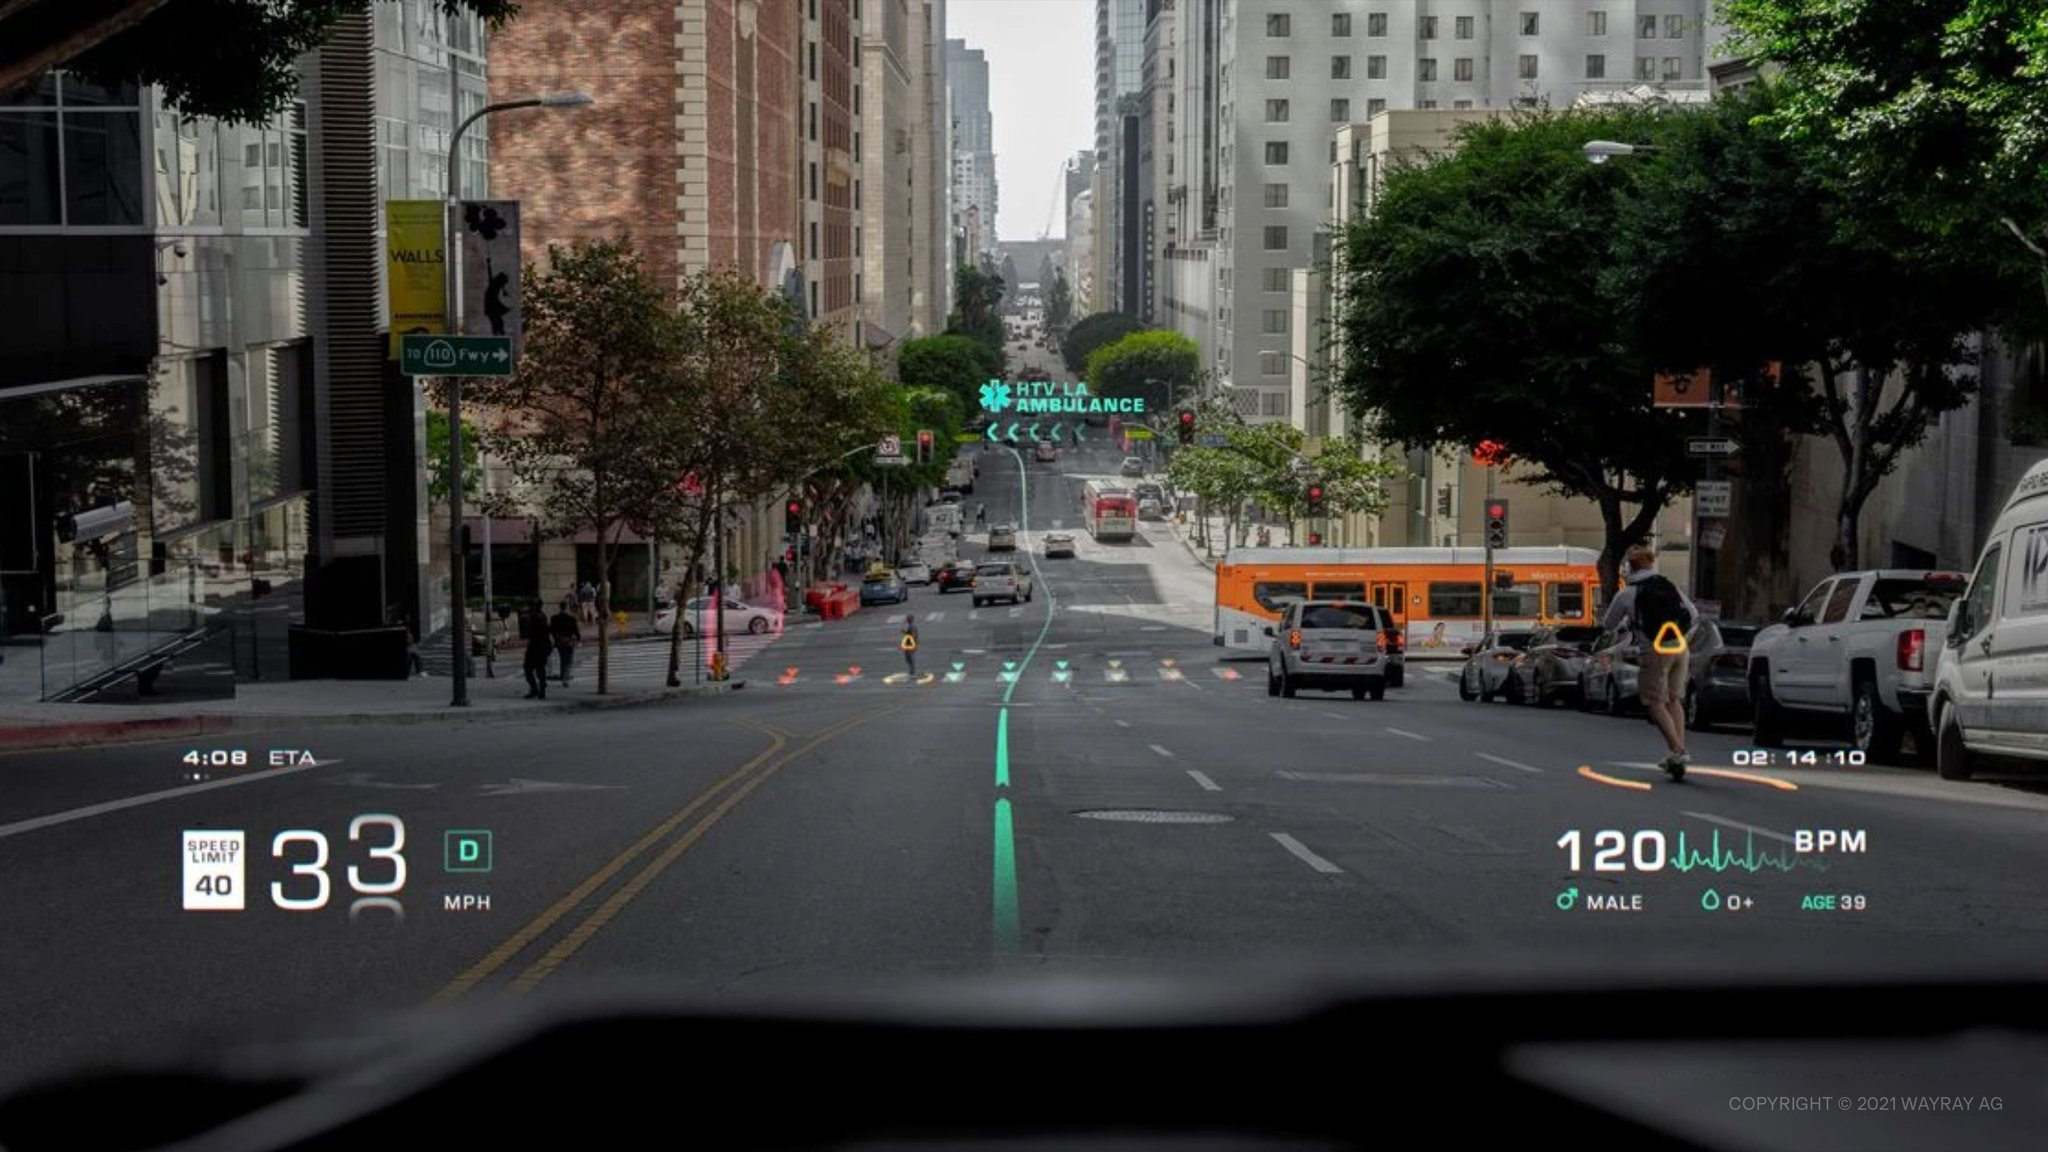
\includegraphics[width=0.6\textwidth]{attachments/wayray.jpg}
    \caption{Das Konzept der in ein Auto integrierten AR-Technologie} \cite{WayRay}
\end{figure}

\subsection{Architektur}
Einer der Vorteile des Einsatzes von AR-Technologie in der Architektur ist die Möglichkeit, dem Nutzer Visualisierungsplattformen für die effektive Verwaltung digitaler Informationen zu bieten. Durch die Integration der AR-Technologie können Architekten Erfahrungen schaffen, die es den Kunden ermöglichen, Entwürfe auf lebensechte Weise zu visualisieren. Dies fördert die Kommunikation zwischen Architekten und Kunden und ermöglicht ein Verständnis des Entwurfs vor Baubeginn. \cite{Chi2013ResearchTA}

Darüber hinaus kann die AR-Technologie auf Baustellen eingesetzt werden, um die Arbeiter bei der Visualisierung von Entwürfen in Räumen zu unterstützen. Dies trägt dazu bei, Fehler zu reduzieren und die Effizienz zu steigern, da die Arbeiter die Platzierung der einzelnen Komponenten genau bestimmen können. Darüber hinaus kann die AR-Technologie Wartungs- und Reparaturanweisungen für Gebäudesysteme bereitstellen, wodurch Ausfallzeiten minimiert und die Sicherheit erhöht werden. \cite{Chi2013ResearchTA}

Ein weiterer Vorteil des Einsatzes von AR-Technologie in der Architektur besteht darin, dass sie den Zugang zu Informationen vor Ort über Dienste ermöglicht. Dies bedeutet, dass Architekten und Bauarbeiter jederzeit und von jedem Ort aus auf projektbezogene Informationen zugreifen können. Eine solche Zugänglichkeit verbessert die Zusammenarbeit zwischen den Teammitgliedern und erleichtert den Arbeitsablauf. \cite{Chi2013ResearchTA}

\subsection{Handel und Marketing}

Augmented Reality wird in der Einzelhandels- und Marketingbranche immer beliebter, um das Kundenerlebnis zu verbessern und die Markentreue zu fördern. Durch den Einsatz von AR können sich die Kunden mit den Produkten auf immersive und personalisierte Weise auseinandersetzen, was zu einer stärkeren Loyalität gegenüber der Marke und höheren Umsätzen führt.

Eine interessante Anwendung der AR-Technologie im Einzelhandel und Marketing ist die Einrichtung von Umkleidekabinen. In diesen virtuellen Räumen können Kunden Kleidung, Accessoires und sogar Make-up anprobieren, ohne in einem Geschäft anwesend zu sein. Unternehmen wie IKEA haben sich diese Technologie zunutze gemacht, um ihren Kunden die Möglichkeit zu geben, sich vor einer Kaufentscheidung ein Bild davon zu machen, wie die Produkte bei ihnen zu Hause aussehen würden. \cite{IKEA_2017}

\vspace{1cm}

\begin{figure}[ht!]
    \centering
    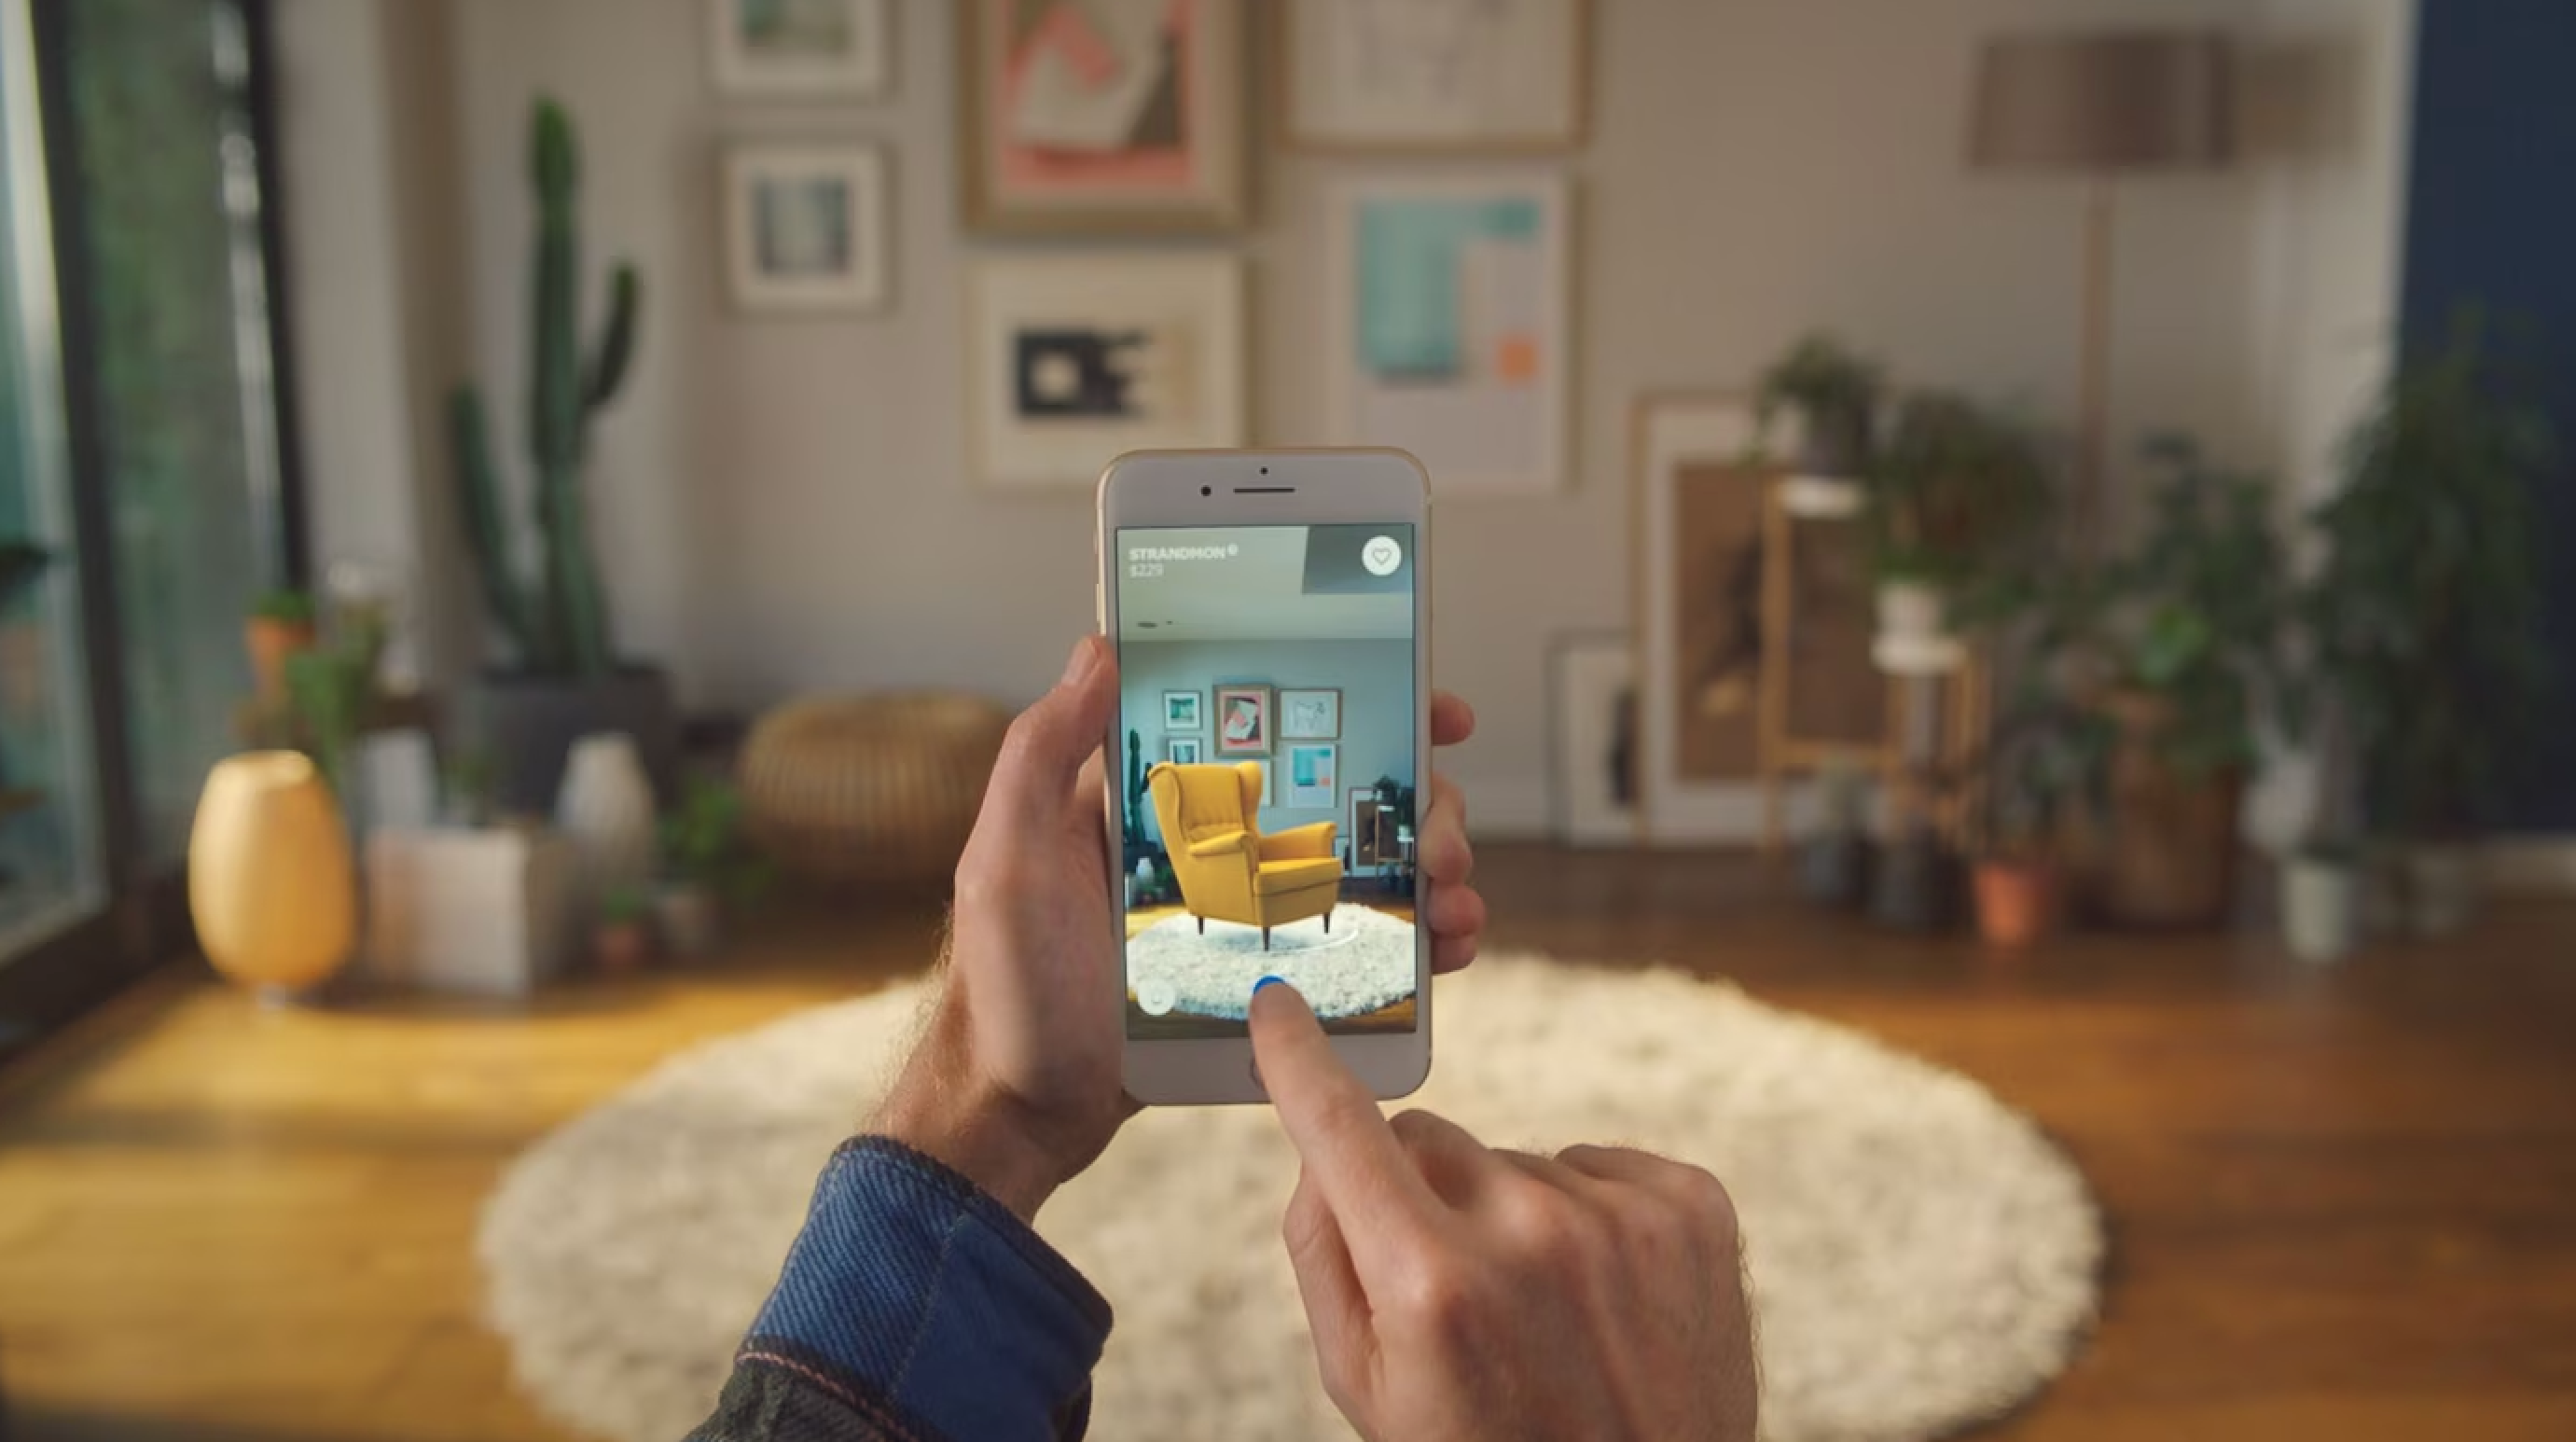
\includegraphics[width=0.6\textwidth]{attachments/ikea.png}
    \caption{IKEA Place im Einsatz} \cite{IKEA_2017}
\end{figure}


Eine weitere Möglichkeit, die AR-Technologie einzusetzen, ist die Visualisierung von Produkten. Sie ermöglicht die Erstellung von 3D-Modellen, mit denen Kunden in einer Umgebung interagieren können. Bekannte Unternehmen wie BMW und Converse nutzen diese Technologie, um ihren Kunden die Möglichkeit zu geben, das Aussehen und die Funktionalität ihrer Produkte in der realen Welt zu erleben \cite{Boeriu_2022}, \cite{Online_Campaigns_2012}

Ausserdem kann die AR-Technologie für standortbezogene Marketingzwecke genutzt werden. Unternehmen haben die Möglichkeit, an bestimmten Orten AR-Erlebnisse zu entwickeln. So könnten sie beispielsweise eine Augmented-Reality-Schnitzeljagd in einem Einkaufszentrum veranstalten oder Informationen über Sehenswürdigkeiten in einer Stadt durch AR bereitstellen.

Zusammenfassend lässt sich sagen, dass die potenziellen Auswirkungen der AR-Technologie auf Handel und Marketing tiefgreifend sind. Indem sie ihren Kunden personalisierte Erlebnisse bieten, können Unternehmen das Engagement erhöhen, die Markentreue fördern und den Umsatz steigern.


